\chapter{Related Work} \label{chap:relatedwork}

Multi-granularity locking is a well-known solution to the problem of hierarchical locking in database systems. 
With MGL, locking a vertex in a hierarchy in a specific mode implicitly locks all its descendants in the same mode. 
This is a powerful concept that allows for efficient locking of hierarchical data structures without the need to lock large portions of the hierarchy.
While powerful, implementing an MGL protocol that successfully achieves this goal is non-trivial. 
The primary challenge is an efficient computation of the ancestor-descendant relationships in the hierarchy. 
Along with this, there are other requirements that contribute to the performance trade-offs of the locking protocol. 


% Generally, any locking approach has certain requirements and balances trade-offs between performance and correctness.
% Hierarchical locking approaches utilize several clever tricks to identify lock granularities, place locks on the vertices of the hierarchy and to ensure that the locking protocol is safe, fair and does not lead to starvation. 

These requirements can be broadly classified into 4 categories:
\begin{itemize}
    \item[\textbf{R1}] Identifying a lock guard for every vertex of a hierarchy.
    \item[\textbf{R2}] Finding an appropriate, optimal lock guard for a request.
    \item[\textbf{R3}] Detecting conflicts between locks i.e. testing ancestor-descendant relationship.
    \item[\textbf{R4}] Housekeeping the metadata required to implement the locking protocol.
\end{itemize}
The different locking approaches discussed in this chapter use different mechanisms to address these requirements with each approach having its own set of trade-offs. 
It would be appropriate to claim that no approach is all encompassing and the choice of the locking approach depends on the specific requirements of the application and the hierarchy being used. 
However, a few locking protocols are more generally suited over others. 

\section{Fixed grain locks}

Fixed grain locks are the simplest form of locking for uses where the hierarchy is known a priori and the semantic classification of the vertices is fixed. 
Fixed grain locking associates a fixed guard for a set of vertices in the hierarchy.
The two extremes of locking discussed in Chapter \ref{chap:background} are variants of fixed grain locking. 
Another approach to fixed grain locking is to associate a lock guard per level of the hierarchy. 
As shown in Figure \ref{fig:level_locks}, the hierarchy is divided into levels and a lock guard is associated with each level. 
In this approach, locking a vertex locks all the other vertices in the same level. 
For example, in Figure \ref{fig:level_locks}, locking vertex $D$ locks vertices $E$, $F$ and $G$ as well since they are in level 2.

\begin{figure}
    \centering
    \captionsetup{justification=centering}
    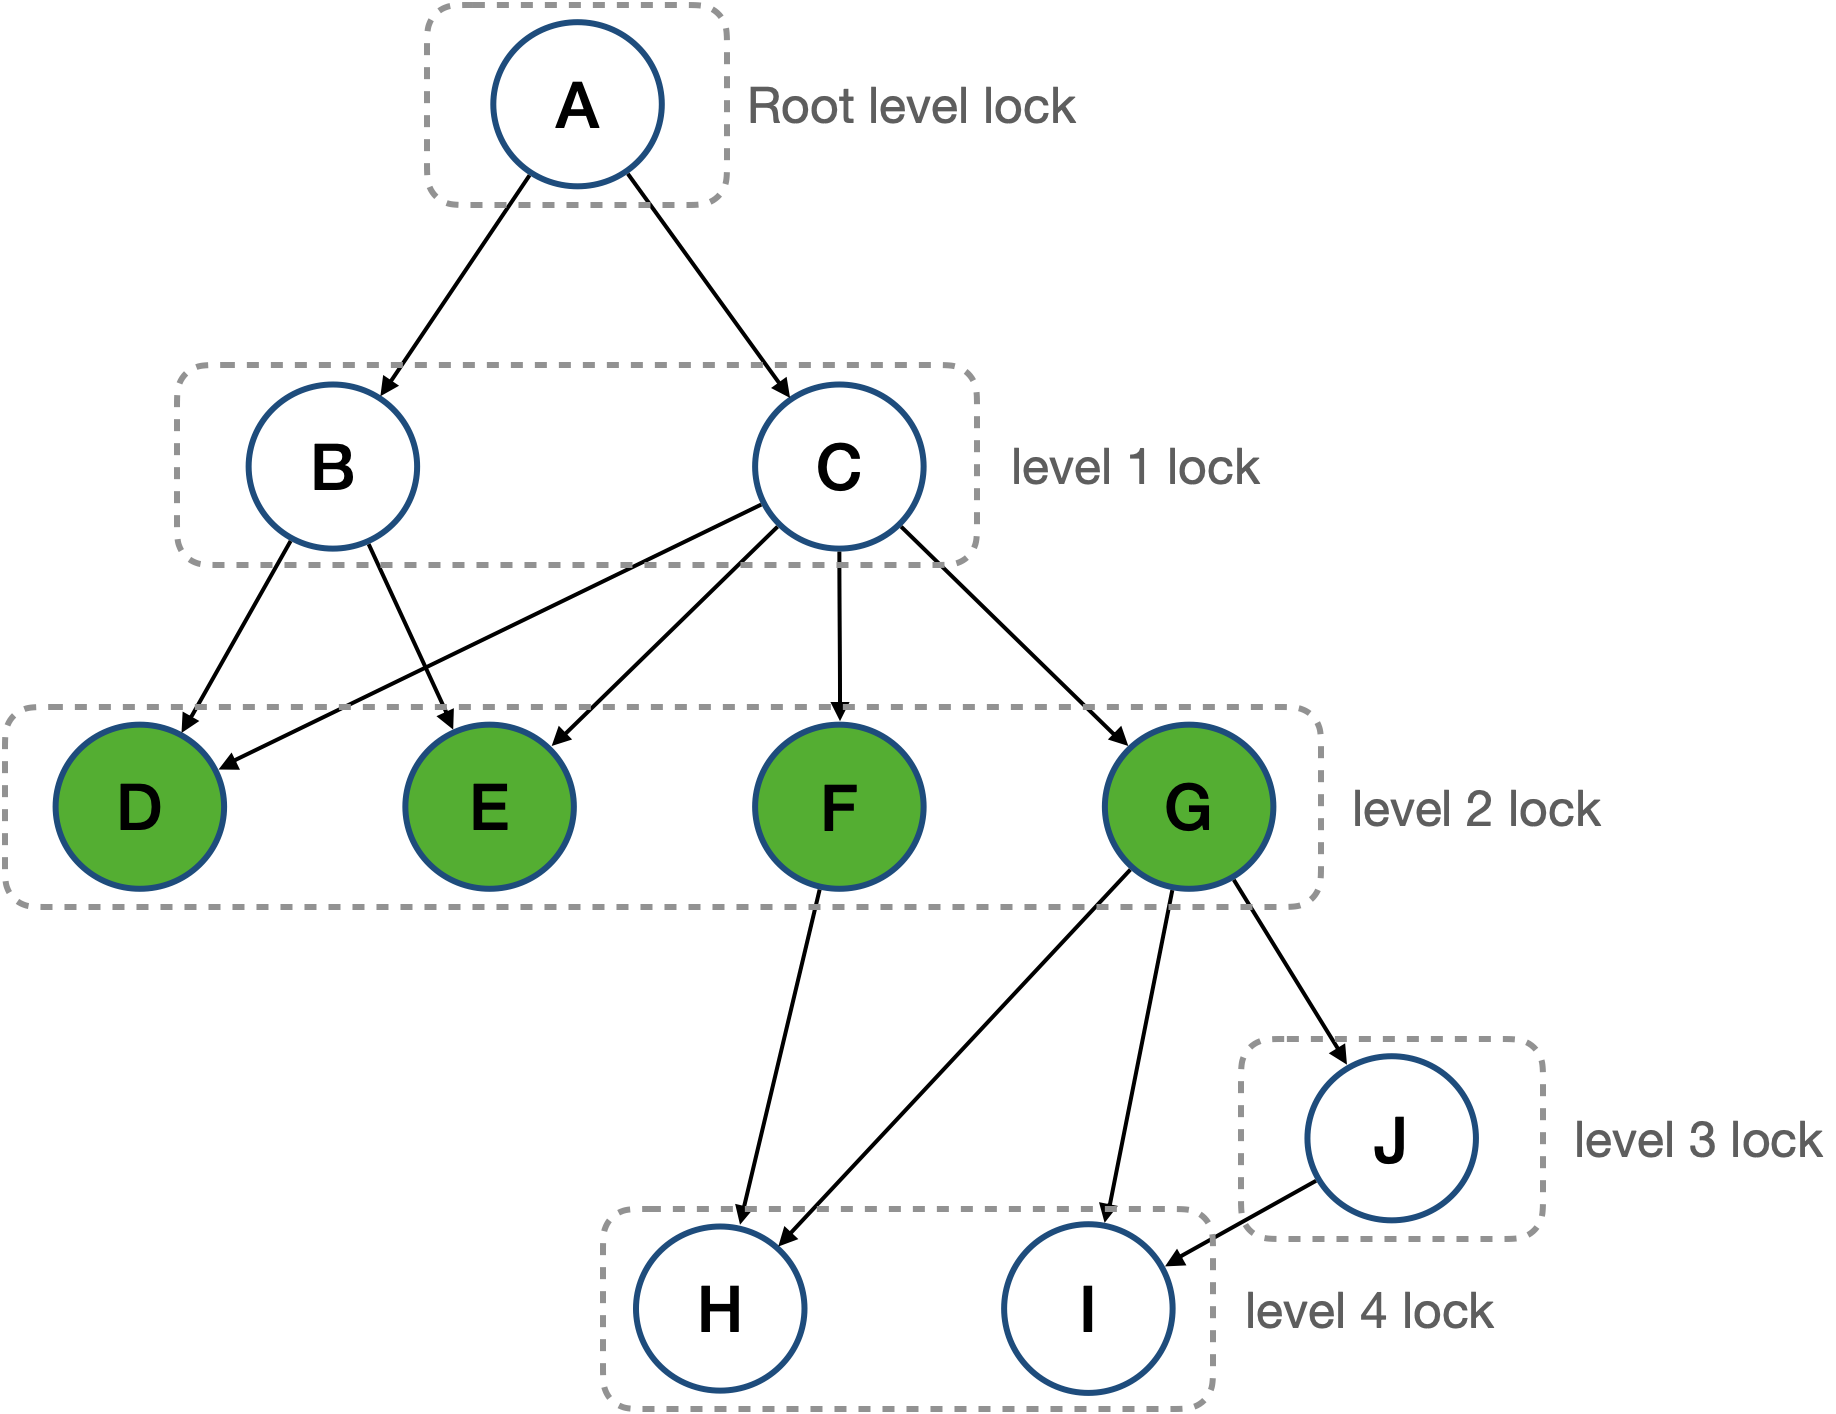
\includegraphics[width=0.7\textwidth]{figures/FixedGrainLevelLocks.png}
    \caption{Hierarchical locks with fixed grains per level and a lock on level 2}
    \label{fig:level_locks}
\end{figure}

Fixed grain locks only fulfil requirement \textbf{R1} since the lock guard is fixed for a set of vertices. 
However, the lock guard is not optimal for any request that does not contain all vertices in a level. 
For example, consider two threads $T_1$ and $T_2$ that want to lock vertices $D$ and $E$ respectively.
Since the lock guard for level 2 is the same, $T_1$ and $T_2$ will conflict with each other. 
However, $D$ and $E$ are not related by an ancestor-descendant relationship and hence should not conflict.

In using fixed grain locks, the lock guard is not optimal. 
Depending on the lock grains chosen, the ancestor-descendant relationship may not be correctly identified. 
This leads to unnecessary conflicts and can lead to performance degradation.

\section{Intention Lock}

Intention locking is one of the first approaches to hierarchical locking that attempts to address the requirements \textbf{R1} and \textbf{R3} with efficiency.
\citet{gray1993granularity} introduced three new lock modes: IS (Intention Shared), IX (Intention Exclusive) and SIX (Shared Intention Exclusive) which signify the intention of a transaction to acquire a shared or exclusive lock on a descendant of a vertex locked under IS, IX or SIX mode respectively.
Table \ref{tab:intention_locks} shows the compatibility matrix for the intention locks.


\begin{table}
    \centering
    \captionsetup{justification=centering}
    \begin{tabular}{c|ccccccc}
        \textbf{Mode} & \textbf{NL} & \textbf{IS} & \textbf{IX} & \textbf{S} & \textbf{SIX} & \textbf{X}\\
        \hline
        \textbf{NL} & \cellcolor{green!25} Y & \cellcolor{green!25} Y & \cellcolor{green!25} Y & \cellcolor{green!25} Y & \cellcolor{green!25} Y & \cellcolor{green!25} Y \\
        \textbf{IS} &  \cellcolor{green!25} Y & \cellcolor{green!25} Y & \cellcolor{green!25} Y & \cellcolor{green!25} Y & \cellcolor{green!25} Y & \cellcolor{red!25} N \\
        \textbf{IX} &  \cellcolor{green!25} Y & \cellcolor{green!25} Y & \cellcolor{green!25} Y & \cellcolor{red!25} N & \cellcolor{red!25} N & \cellcolor{red!25} N \\
        \textbf{S} &  \cellcolor{green!25} Y & \cellcolor{green!25} Y & \cellcolor{red!25} N & \cellcolor{green!25} Y & \cellcolor{red!25} N & \cellcolor{red!25} N \\
        \textbf{SIX} &  \cellcolor{green!25} Y & \cellcolor{green!25} Y & \cellcolor{red!25} N & \cellcolor{red!25} N & \cellcolor{red!25} N & \cellcolor{red!25} N \\
        \textbf{X} &  \cellcolor{green!25} Y & \cellcolor{red!25} N & \cellcolor{red!25} N & \cellcolor{red!25} N & \cellcolor{red!25} N & \cellcolor{red!25} N \\
    \end{tabular}
    \caption{Compatibility matrix for intention lock modes. \textbf{NL}: NoLock, \textbf{IS}: Intention Shared, \textbf{IX}: Intention Exclusive, \textbf{S}: Shared, \textbf{SIX}: Shared Intention Exclusive, \textbf{X}: Exclusive}
    \label{tab:intention_locks}
\end{table}



\begin{figure}[h]
    \centering
    \captionsetup{justification=centering}
    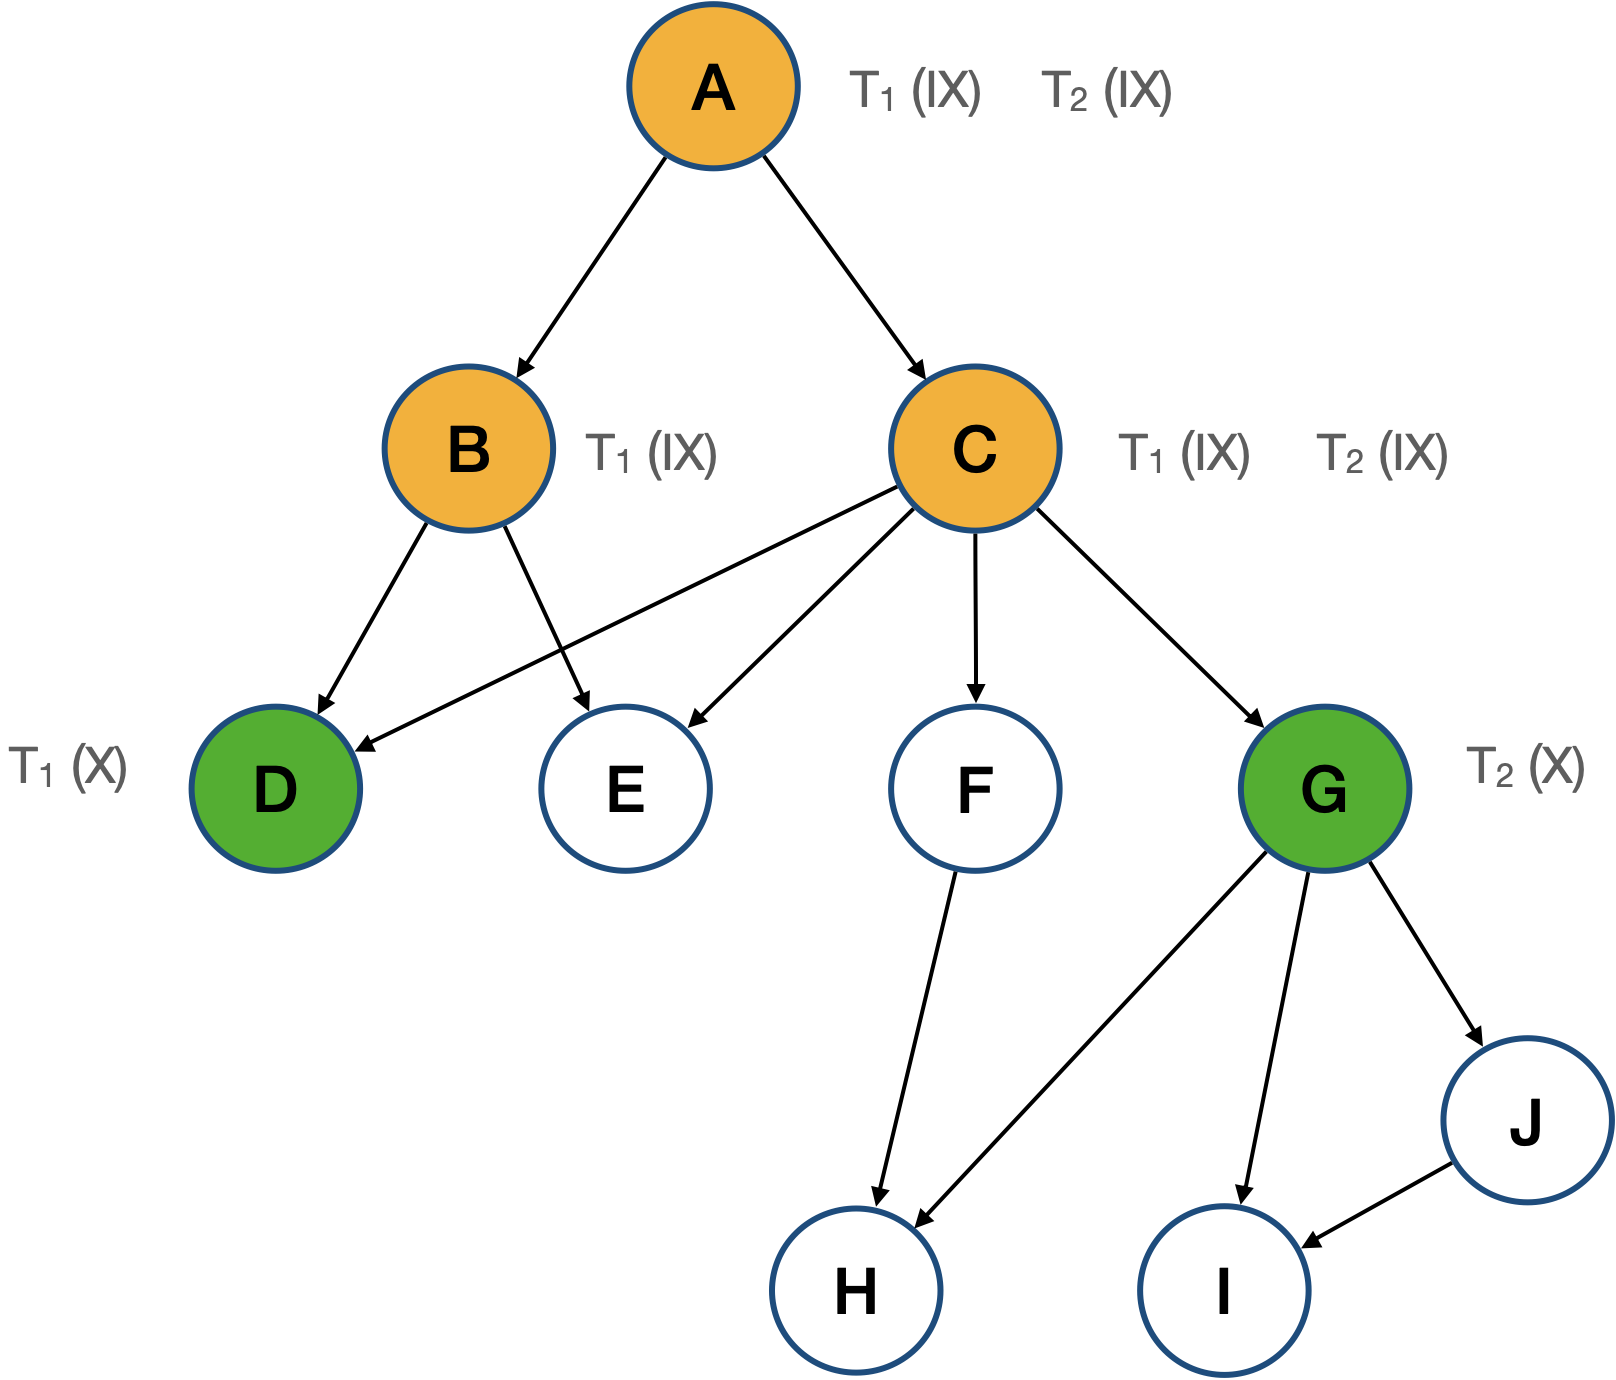
\includegraphics[width=0.5\textwidth]{figures/IntentionLockExample.png}
    \caption{Multi granularity locking via Intention locks. \\ $T_1$ takes an exclusive lock on vertex $D$ and $T_2$ takes an exclusive lock on vertex $G$ }
    \label{fig:intention_lock_example}
\end{figure}

Consider the example in figure \ref{fig:intention_lock_example} where a transaction $T_1$ takes an exclusive lock on vertex $D$ and another thread, $T_2$ takes an exclusive lock on vertex $G$. 
Since $D$ and $G$ are not related by an ancestor-descendant relationship, they should not conflict.
To achieve this with intention locks, both threads start from the root i.e $A$ and place intention tags on the vertices from the root to their lock targets i.e $D$ and $G$ respectively. 
Let's assume that $T_1$ is faster than $T_2$ and manages to acquire its locks first. 
$T_1$ takes $IX$ on vertices $A$, $B$ and $C$; in this order, and then takes an exclusive lock on $D$. 

When $T_2$ tries to acquire a lock on $G$, it places $IX$ on vertices $A$, $B$ and $C$;in this order, as well, before trying to acquire a lock on $G$. 
When $T_2$ tries to acquire a lock on $A$, it detects a pre-existing  $IX$ lock. 
Since two $IX$ locks are compatible, as seen in Table \ref{tab:intention_locks}, $T_2$ can acquire the $IX$ lock on $A$.
Similarly, $T_2$ can acquire the $IX$ lock on $C$ and then proceed to acquire the exclusive lock on $G$.


The process of acquiring locks in this manner guarantees that the ancestor-descendant relationship is correctly identified. 
However, it involves multiple traversals from the root to the lock target. 
In the example in Figure \ref{fig:intention_lock_example}, $T_1$ performs the following two traversals:

\begin{itemize}
    \item $A \rightarrow B \rightarrow D$
    \item $A \rightarrow C \rightarrow D$
\end{itemize}

With trees, every vertex is reachable from the root via a unique path. 
This, however, is not the case with general graphs.
In general graphs, as the number of paths from the root to a vertex increases, the number of traversals required to acquire a lock on that vertex also increases.
This leads to a significant performance degradation. 

So, while intention locks fulfil requirements $R1$ and $R2$, requirements $R3$ incurs a significant performance penalty. 

\section{DomLock}

Dominator based locking (DomLock) \cite{kalikar2016domlock} uses dominators to identify the ancestor descendant relationship in a hierarchy. DomLock finds a partial ordering of vertices in the hierarchy based on the ancestor-descendant relationship between them. To this end, DomLock uses the concept of dominators and immediate dominators. 
\begin{definition}[Dominator]
    A vertex $d$ is a dominator of another vertex $v$ if all the paths from root to $v$ pass through d.
\end{definition}

\begin{definition}[Immediate Dominator]
    Immediate Dominator: A dominator d is an immediate dominator of another vertex $v$ if there exists no other dominator for $v$ on the paths between d and $v$.
\end{definition}

\subsection{Labelling through numeric intervals}
In order to identify the dominators of a vertex more efficiently, DomLock uses a labelling scheme that assigns a pair of integers to each vertex. This pair is called the \emph{interval} of the vertex. The interval of a vertex $v$ is denoted as $[lv, rv]$. 
The interval of a vertex $v$ is such that $lv \leq lu$ and $rv \geq ru$ for all vertices $u$ that are descendants of $v$. 

These intervals are computed by performing a depth-first traversal of the hierarchy. Consider the example in figure \ref{fig:domlock_example_locked}. The leaves of the hierarchy are labelled with unit intervals. For example, vertex $D$ is labelled with the interval $[1, 1]$ since it is the first vertex in the DFS traversal. 
\begin{figure}
    \centering
    \captionsetup{justification=centering}
    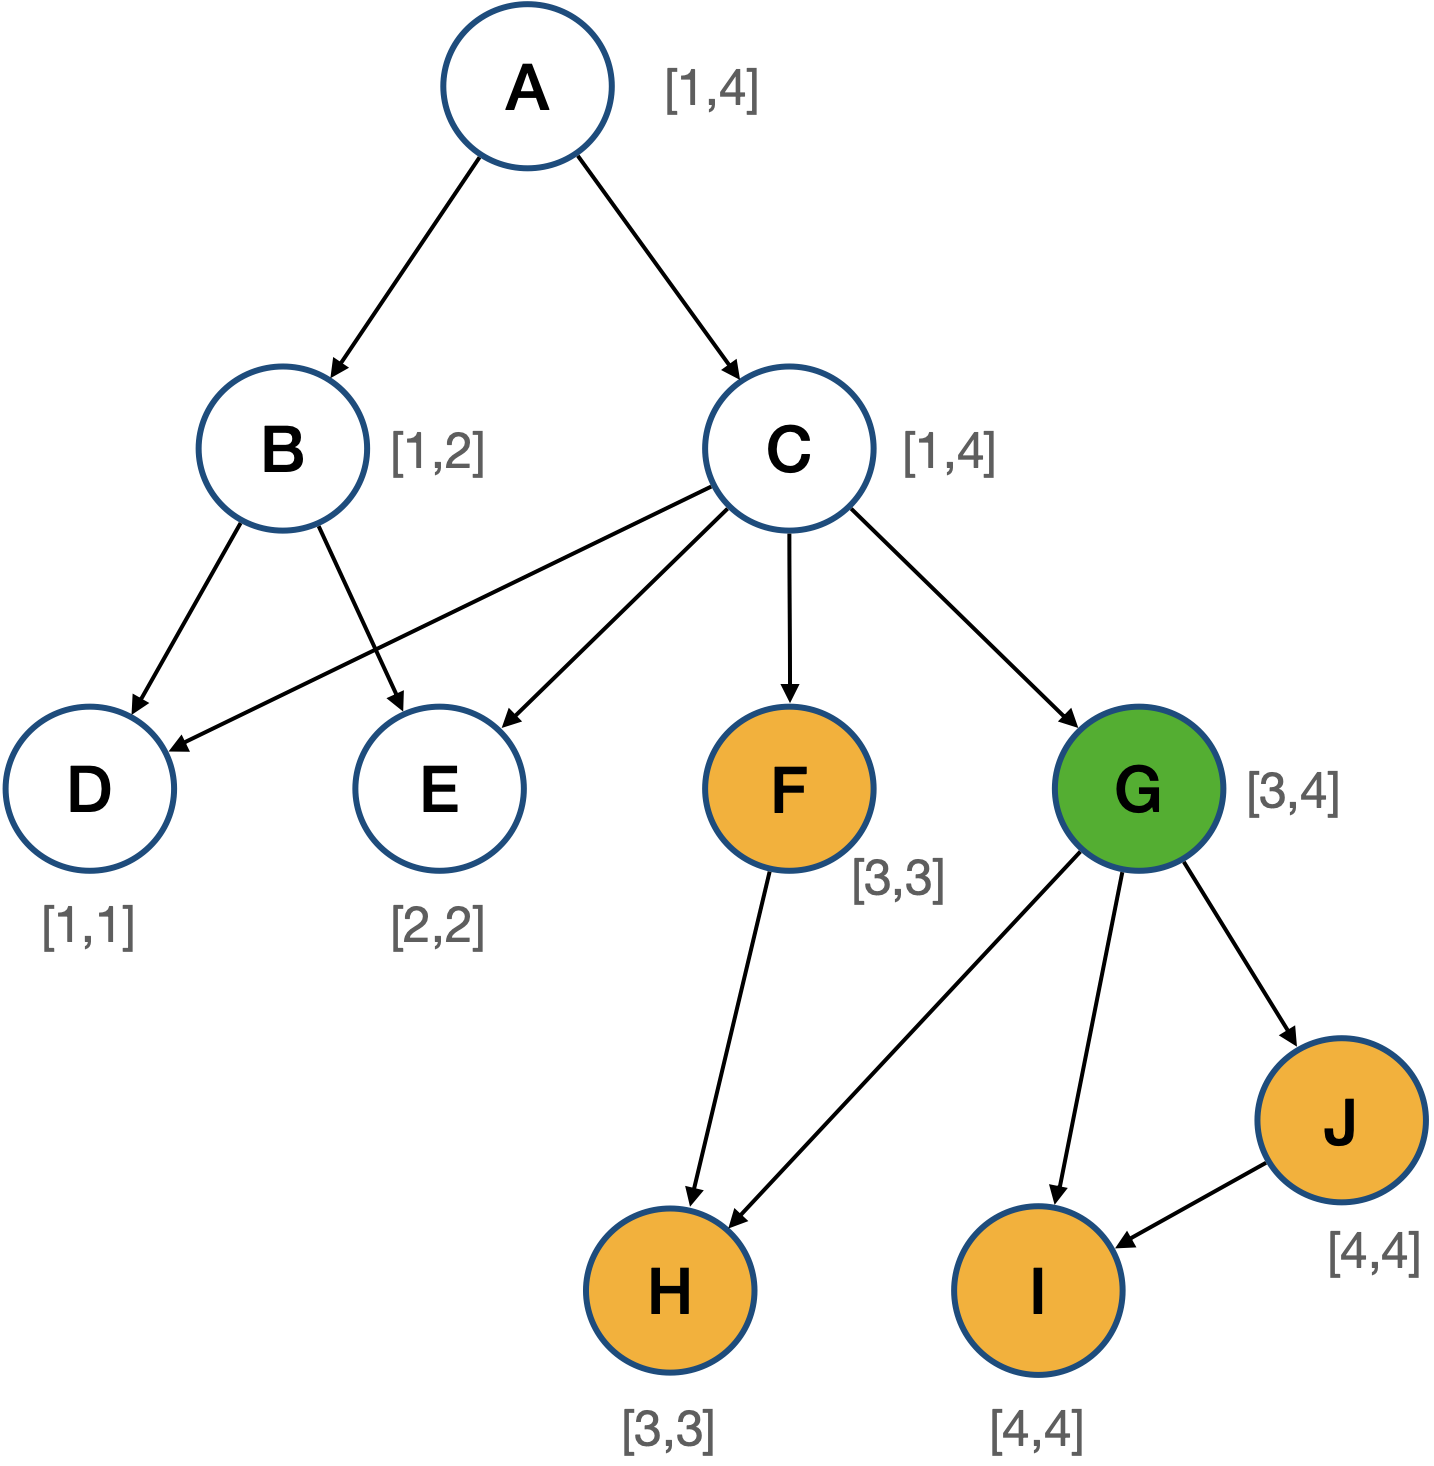
\includegraphics[width=.5\textwidth]{figures/domlock_example_with_lock.png}
    \caption{Hierarchy labelled with DomLock intervals and DomLock on $G$ (lock guard) with the grain of the grain of the lock (yellow).}
    \label{fig:domlock_example_locked}
\end{figure}
For an internal vertex, the interval is computed via the intervals of its children. The $lv$ value of an internal vertex $v$ is the minimum of the $l$ values of its children. The $rv$ value of an internal vertex $v$ is the maximum of the $r$ values of its children. For example, in figure \ref{fig:domlock_example_locked}, vertex $G$ has three children $H$, $I$ and $J$. The interval of $G$ is $[3,4]$ since the minimum $l$ value of its children is 3 and the maximum $r$ value of its children is 4. The computation of intervals is done in a bottom-up fashion via a post-order traversal of the hierarchy. 
% \begin{figure}[h]
%     \centering
%     \captionsetup{justification=centering}
%     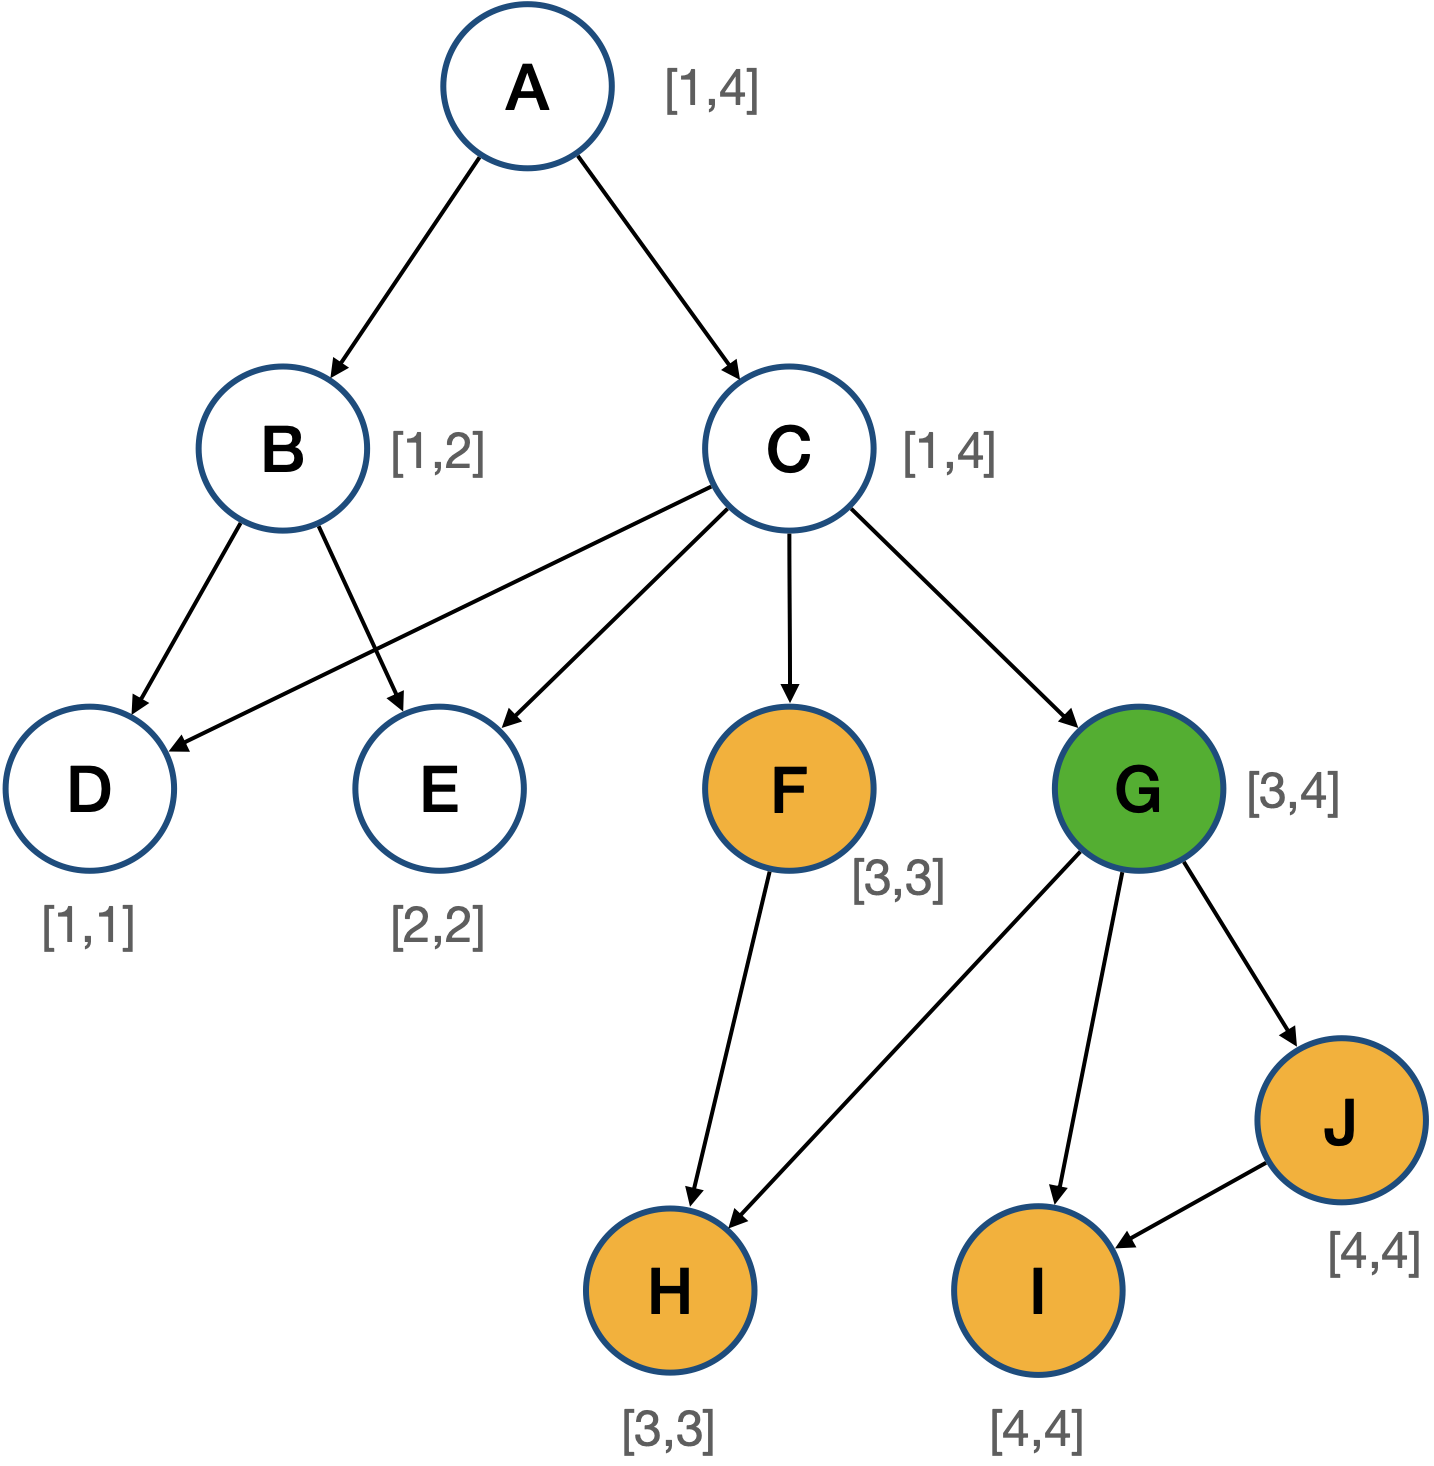
\includegraphics[width=0.5\textwidth]{figures/domlock_example_with_lock.png}
%     \caption{DomLock on guard $G$ with the grain of the grain of the lock (yellow).}
%     \label{fig:domlock_example_locked}
% \end{figure}

\subsection{Lock Grain identification}
The intervals of the vertices are used to check subsumption. A vertex $u$ subsumes another vertex $v$ when their intervals overlap i.e. $lv \leq ru \land lu \leq rv$. The lock grain of a guard $u$ is the set of vertices that have an overlapping interval with the interval of $u$. So, in figure \ref{fig:domlock_example_locked}, $G$ subsumes $F$, $H$, $I$ and $J$ since the interval of $G$ overlaps with the the intervals of $F$, $H$, $I$ and $J$ which are $[3,3]$, $[3,3]$, $[4,4]$ and $[4,4]$ respectively.

Herein lies the first major drawback of DomLock. \emph{False subsumptions} occur when the intervals of two vertices overlap but they are not related by an ancestor-descendant relationship. For example, in figure \ref{fig:domlock_example_locked}, $G$ is the dominator of $F$ but $F$ is not a descendant of $G$. Sometimes, due to false subsumptions disjoint subgraphs are locked together. This leads to spurious lock conflicts and consequently, performance degradation. 

\subsection{Label recomputation}
Another drawback of DomLock is that it does not support dynamic hierarchies. The intervals of the vertices are computed once via a post-order traversal. When a vertex is added or removed from the hierarchy, this computation has to be redone. 

\begin{figure}[h]
    \centering
    \captionsetup{justification=centering}
    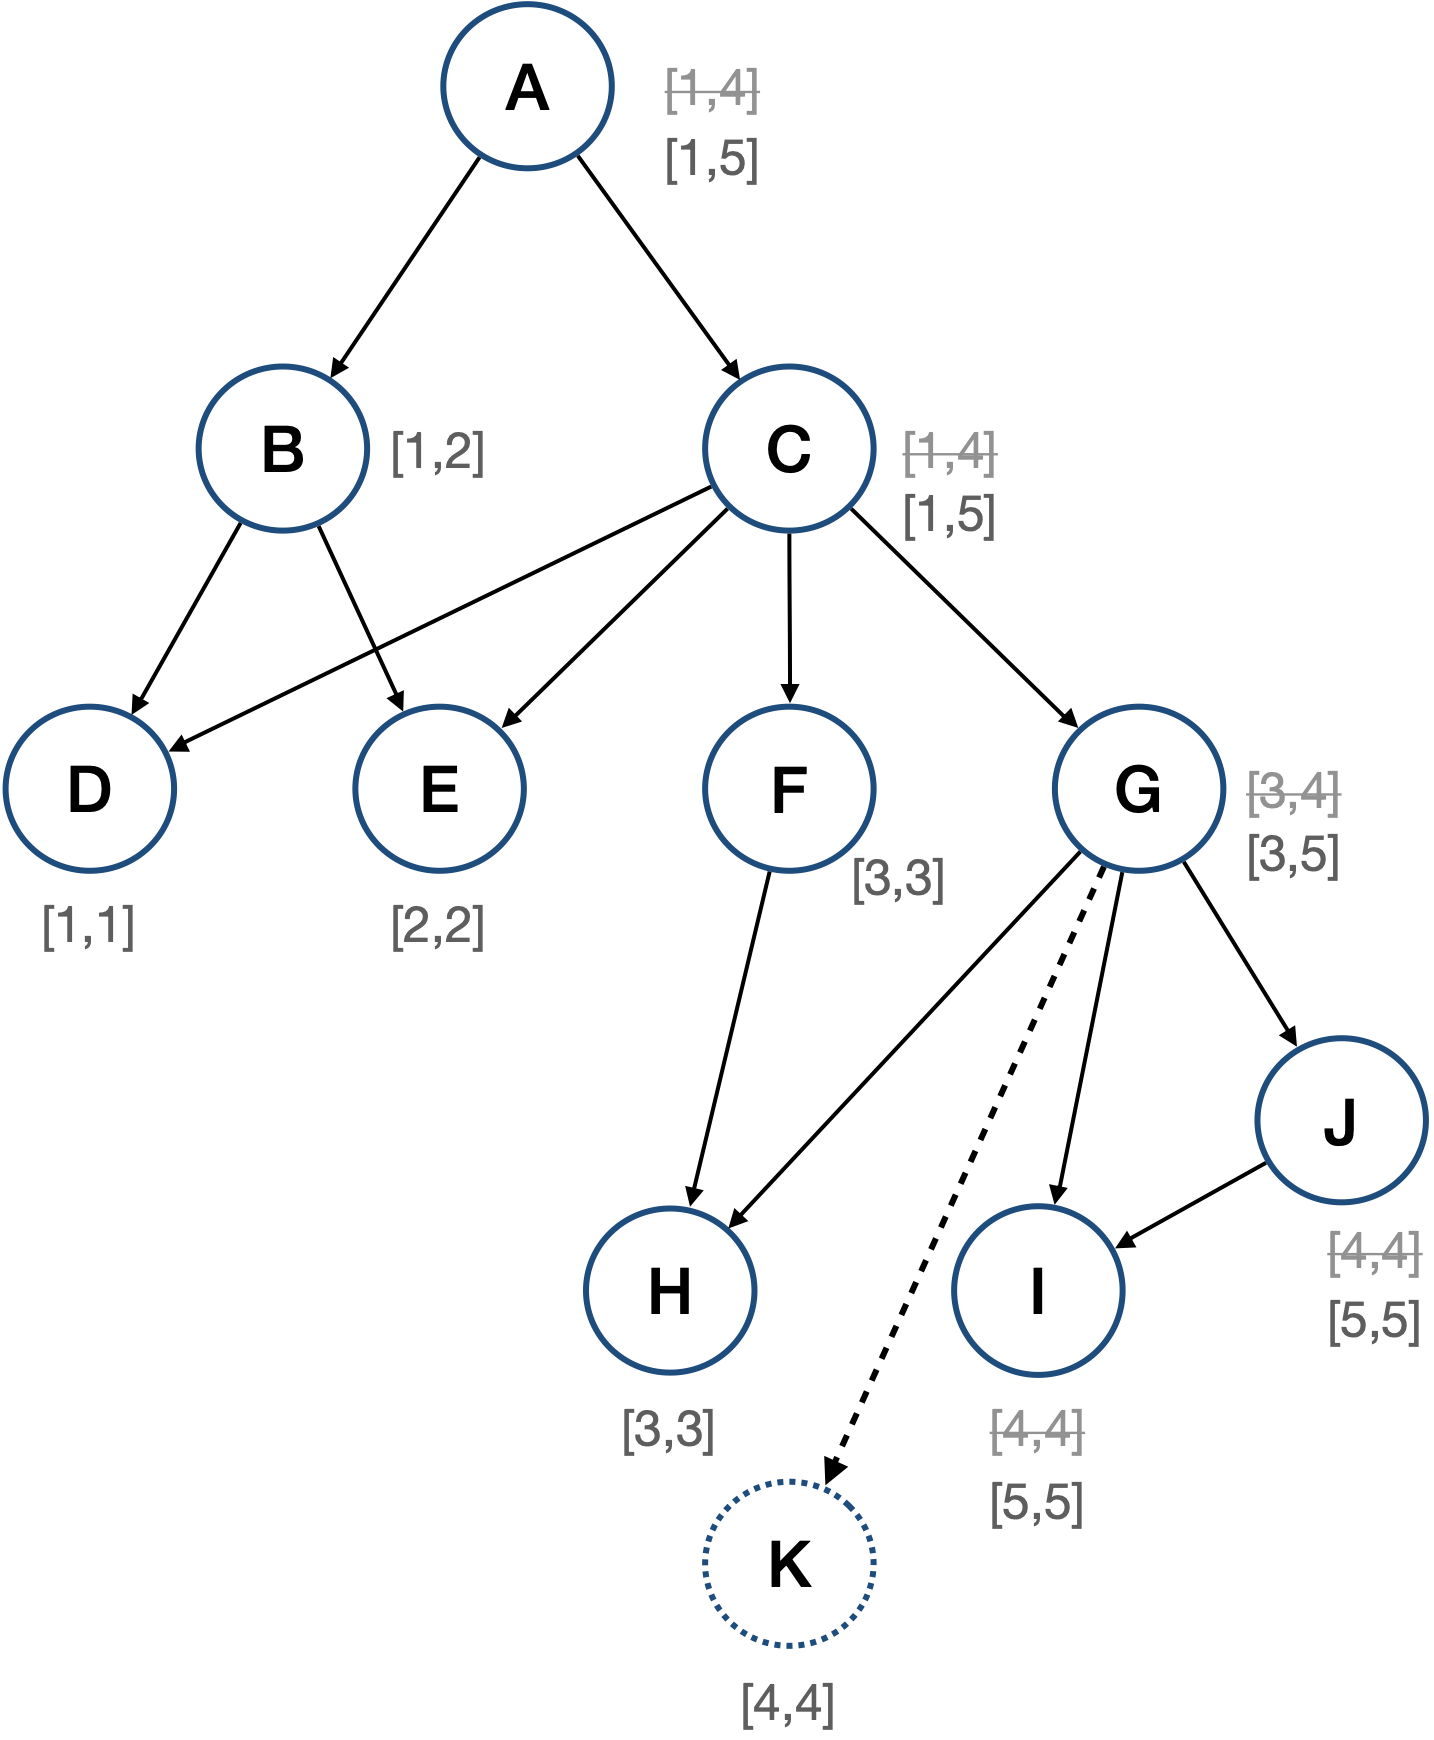
\includegraphics[width=0.5\textwidth]{figures/domlock_example_with_SM.png}
    \caption{DomLock interval recomputation for a vertex insertion}
    \label{fig:domlock_example_SM}
\end{figure}

For example, consider the hierarchy in figure \ref{fig:domlock_example_SM}. If a vertex $K$ is added as a child of $G$ after $H$, $K$ gets the interval $[4,4]$. $I$ and $J$ get the interval $[5,5]$. Following this, the interval of $G$ is recomputed as $[3,5]$. This recomputation has to be done for all the ancestors of $G$ as well, which includes the root of the hierarchy. In order to prevent concurrent reads from interfering with the recomputation, a lock has to be placed on the root of the hierarchy. This lock is held until the recomputation is complete. 
In dynamic hierarchies, such modifications can lead to a significant performance penalty due to the lack of parallelism in the relabelling. 

While DomLock addresses requirements $R1$ and $R2$, false subsumptions and the lack of support for dynamic hierarchies incur significant penalties against requirement $R3$ and $R4$ respectively.



\section{Multi Interval DomLock (MID)}
Multi Interval DomLock \cite{anjuMID} is a successor to DomLock which uses a pair of intervals on each vertex to identify the dominator. MID maintains in addition to the DomLock intervals, another interval computed by a reverse post-order traversal of the hierarchy called the \emph{'DFS-on-image'}. Figure \ref{fig:MID_example_locked} shows the MID intervals for a hierarchy. 

\subsection{Labeling through a pair of numeric intervals}

Each vertex is labelled with two intervals: the DomLock interval and the MID interval. The only difference between the two intervals is the order of traversal of vertices. DomLock intervals being post-order and MID intervals being reverse post-order. Like DomLock, the interval of a leaf is a unit.
% \begin{figure}[h]
%     \centering
%     \captionsetup{justification=centering}
%     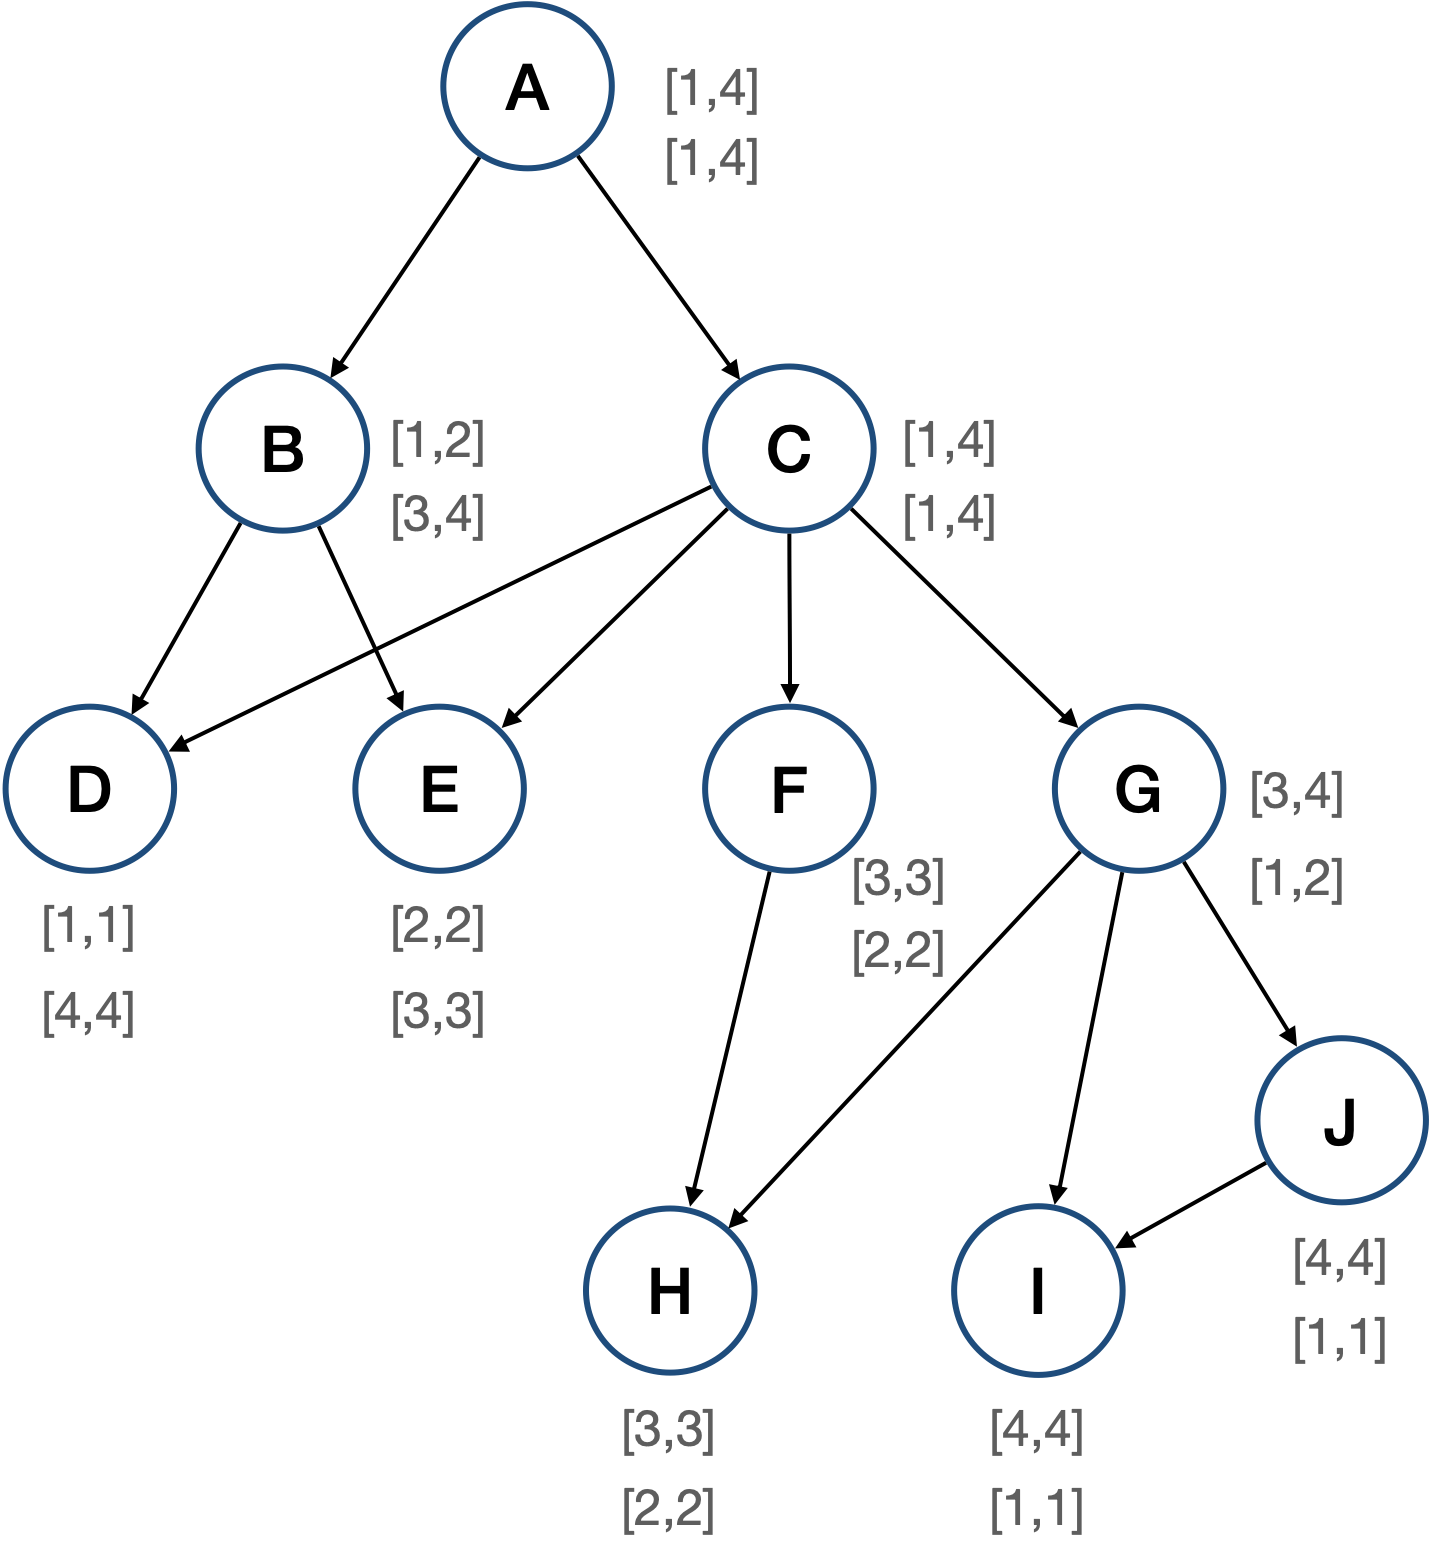
\includegraphics[width=0.5\textwidth]{figures/MID_example.png}
%     \caption{Hierarchy labelled with a pair of intervals: DomLock (top) and MID (bottom)}
%     \label{fig:MID_example}
% \end{figure}

For example, in figure \ref{fig:MID_example_locked} , vertex $H$ is labelled with a second interval $[2,2]$ in addition to the DomLock interval $[3,3]$ since it is the second vertex in the reverse post-order traversal. Again, like DomLock, for an internal vertex, the interval is computed via the intervals of its children. For both intervals, the $l(v)$ value of an internal vertex $v$ is the minimum of the $l$ values of its children. The $r(v)$ value of an internal vertex $v$ is the maximum of the $r$ values of its children. For example, in figure \ref{fig:MID_example_locked}, vertex $G$ has three children $H$, $I$ and $J$. The intervals of $G$ are $[3,4]$ and $[1,2]$ for DomLock and MID respectively since the minimum $l$ value of its children is 3 and 1 and the maximum $r$ value of its children is 4 and 2 respectively.

\subsection{Lock Grain identification}

The two pairs of intervals are used in an attempt to reduce \emph{false subsumptions} where a vertex subsumes its siblings. When testing subsumption in MID, the two intervals are tested for overlap. A vertex $v$ with intervals $[vl_1, vr_1]$ and $[vl_2, vr_2]$, subsumes another vertex $u$ with intervals $[ul_1, ur_1]$ and $[ul_2, ur_2]$ iff $vl_1 \leq ur_1 \land ul_1 \leq vr_1 \land vl_2 \leq ur_2 \land ul_2 \leq vr_2$.

\begin{figure}[H]
    \centering
    \captionsetup{justification=centering}
    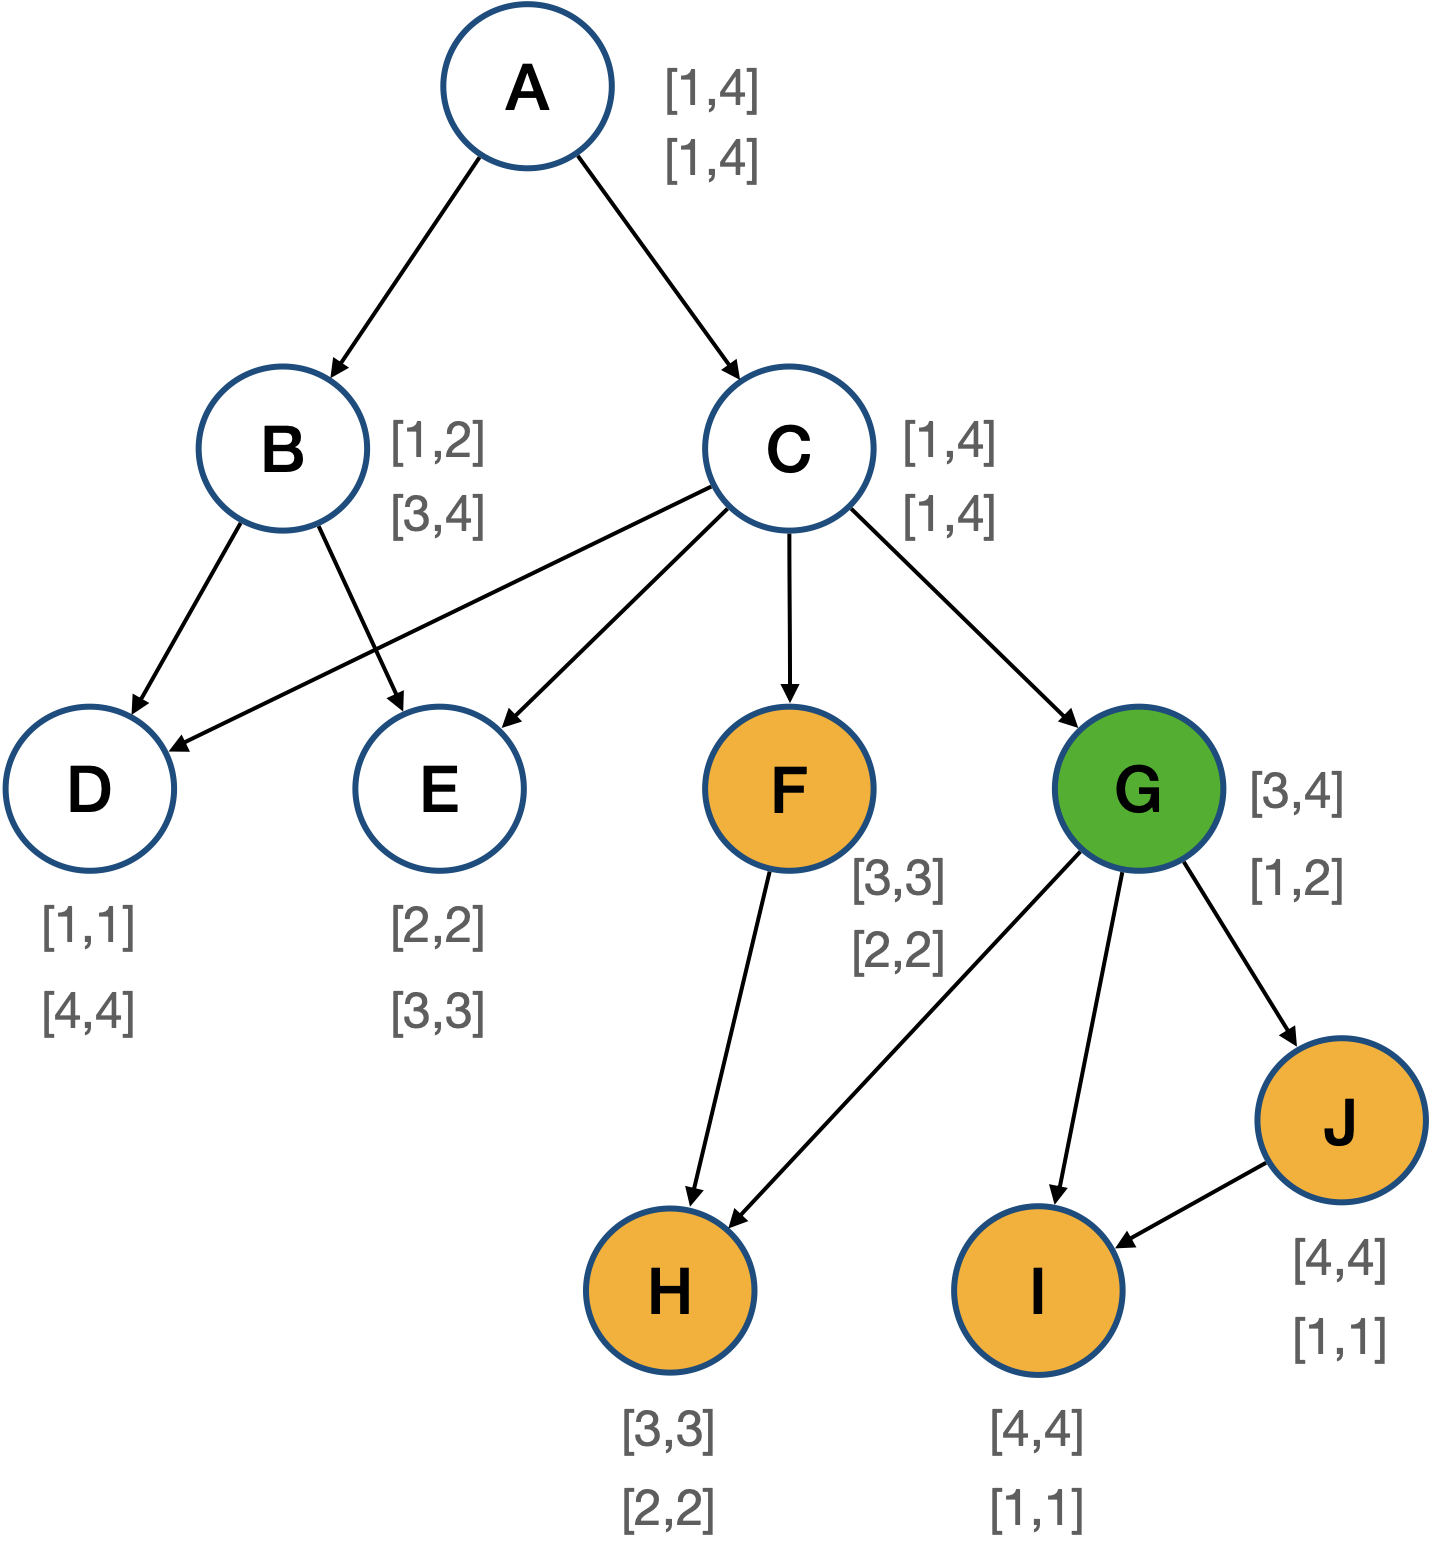
\includegraphics[width=0.5\textwidth]{figures/MID_example_with_lock.png}
    \caption{MID labels with lock on guard $G$ with the grain of the lock (yellow)}
    \label{fig:MID_example_locked}
\end{figure}

For example in figure \ref{fig:MID_example_locked}, $G$ subsumes $F$, $H$, $I$ and $J$ since both intervals of $G$ overlap with the respective intervals of $F$, $H$, $I$ and $J$. However, we still encounter a false subsumption. $G$ subsumes $F$ but $F$ is not a descendant of $G$. Like DomLock, MID also suffers from poor performance due to such spurious conflicts.

\subsection{Label recomputation}
MID encounters double the penalty for recomputing vertex labels in dynamic hierarchies when a structural modification occurs. In DomLock, a single post-order-traversal is enough to compute the intervals so a structural modification leads to the recomputation of intervals in a single traversal. In MID, two traversals are required to compute the intervals. As a consequence, the intervals of all vertices is often recomputed. 

\begin{figure}[H]
    \centering
    \captionsetup{justification=centering}
    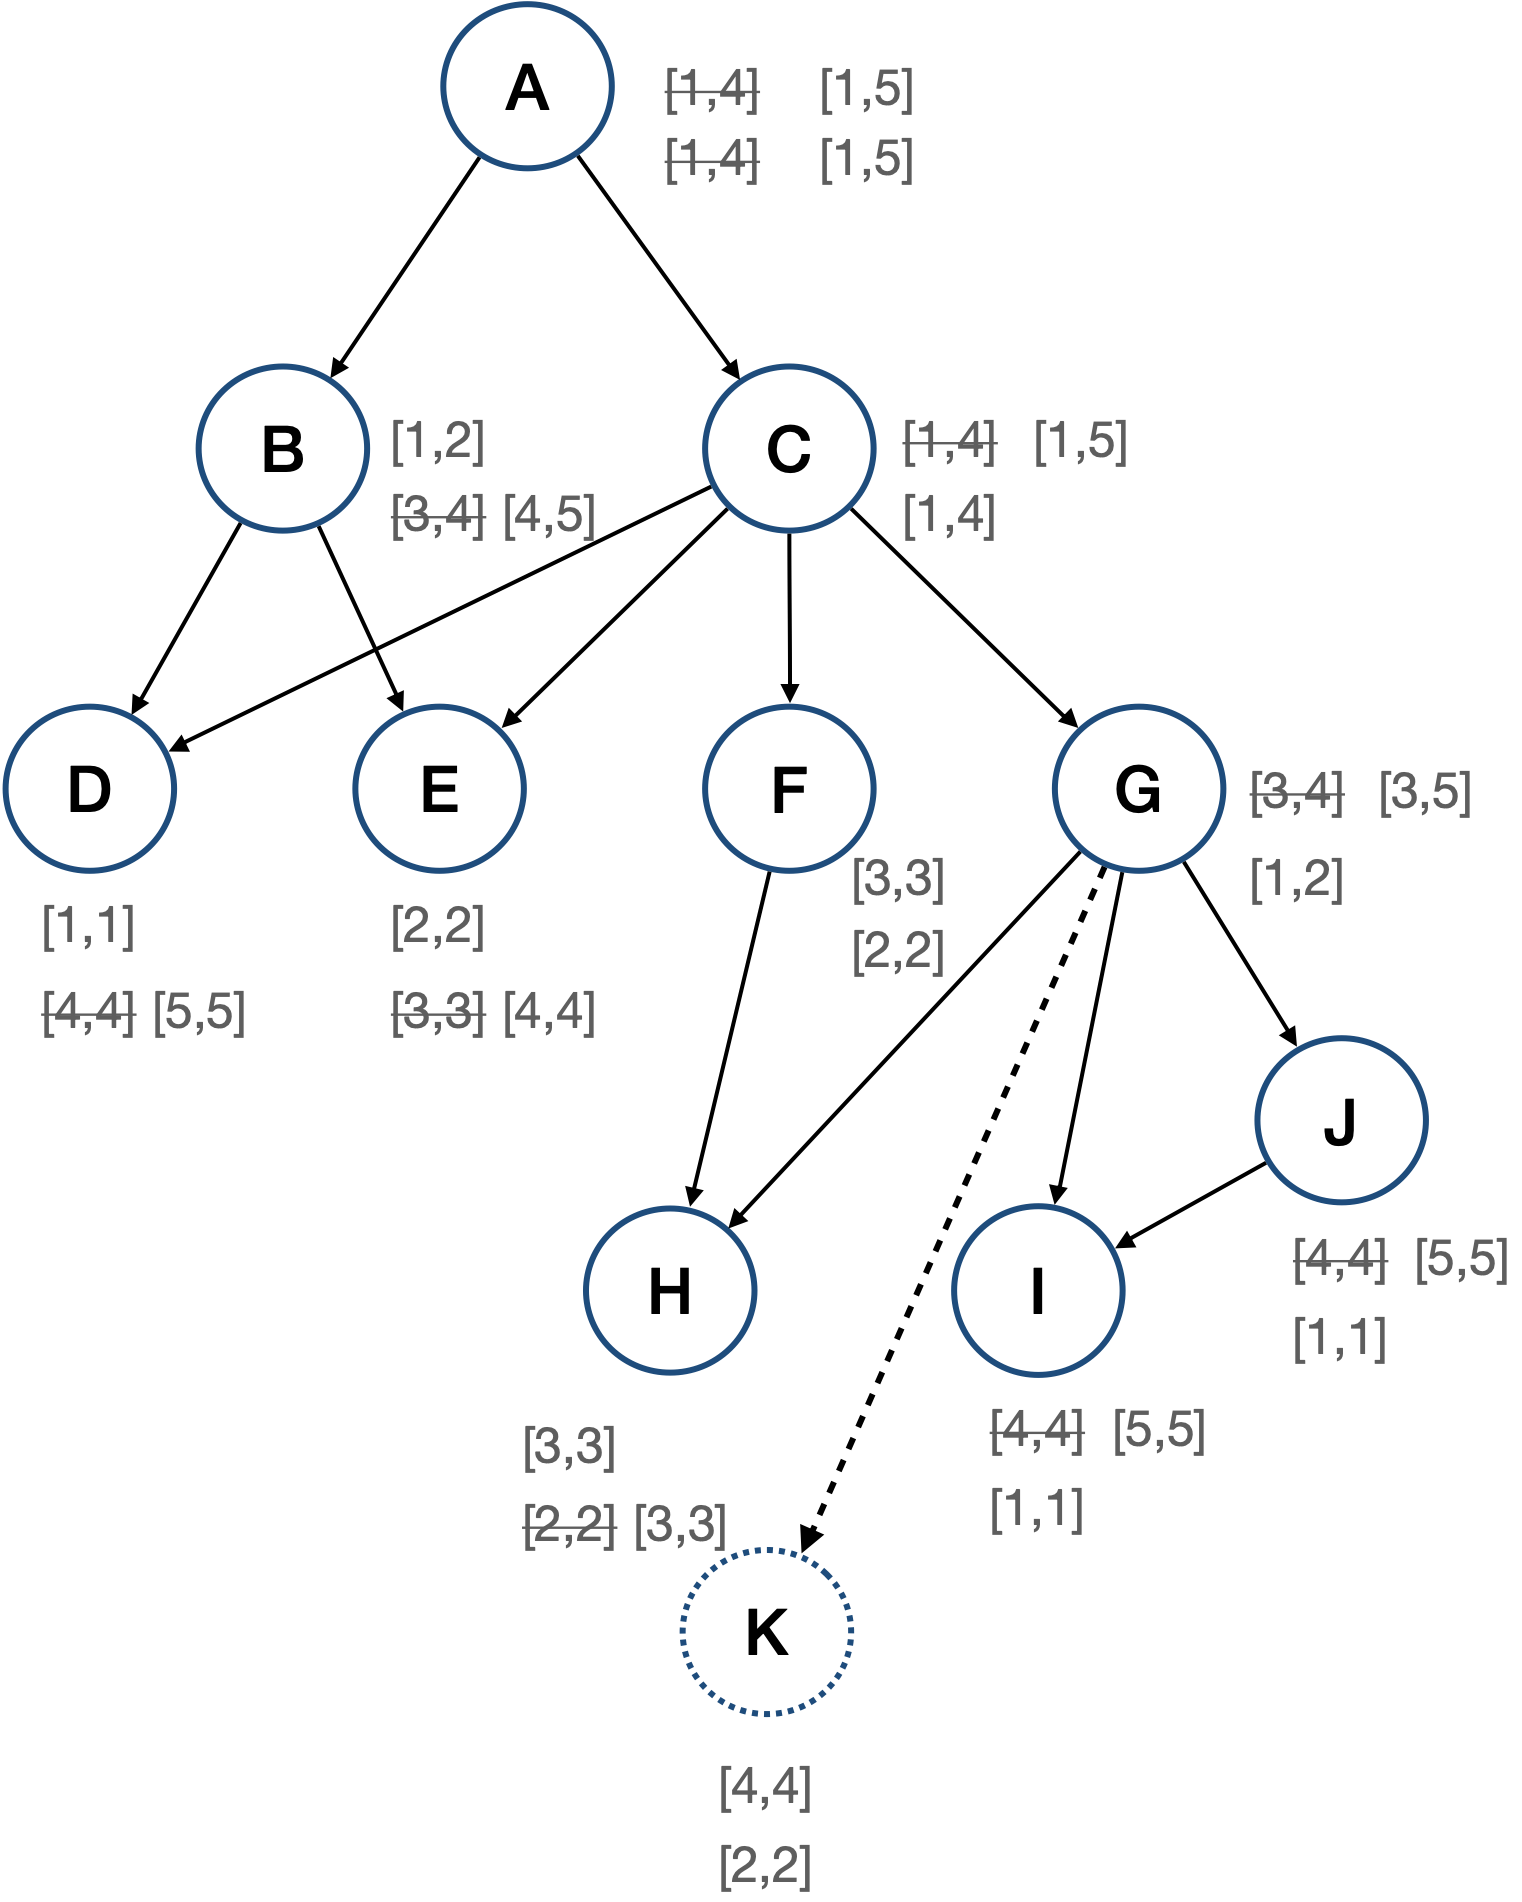
\includegraphics[width=0.5\textwidth]{figures/MID_example_with_SM.png}
    \caption{MID interval recomputation for a vertex insertion}
    \label{fig:MID_example_SM}
\end{figure}

For example, when a vertex $K$ is inserted as a child of $G$ as shown in figure \ref{fig:MID_example_SM}, At least one interval for every vertex is recomputed. These intervals are then propagated to the root of the hierarchy. In order to prevent concurrent reads from interfering with the recomputation, a lock has to be placed on the root of the hierarchy. This lock is held until the recomputation is complete. This lock is essentially a mutex, restricting concurrency.

MID tries to eliminate false subsumptions present in DomLock but does not do so successfully. The performance penalty for recomputation in dynamic hierarchies is doubled in MID. As such, MID fulfils requirements $R1$ and $R2$ but incurs even more penalties against requirements $R3$ and $R4$ than DomLock.

\section{Flexible granularity Locking (FlexiGran)}
FlexiGran \cite{FlexiGran2024} aims to enable the existence of MGL and fixed grain locks on the same hierarchy. The fixed grain locks used by flexigran are fine grained i.e. every vertex is its own guard. FlexiGran uses the intervals of DomLock  as vertex labels and uses vertex depth to determine ancestor-descendent relationships between two identical intervals.
\begin{figure}
    \centering
    \captionsetup{justification=centering}
    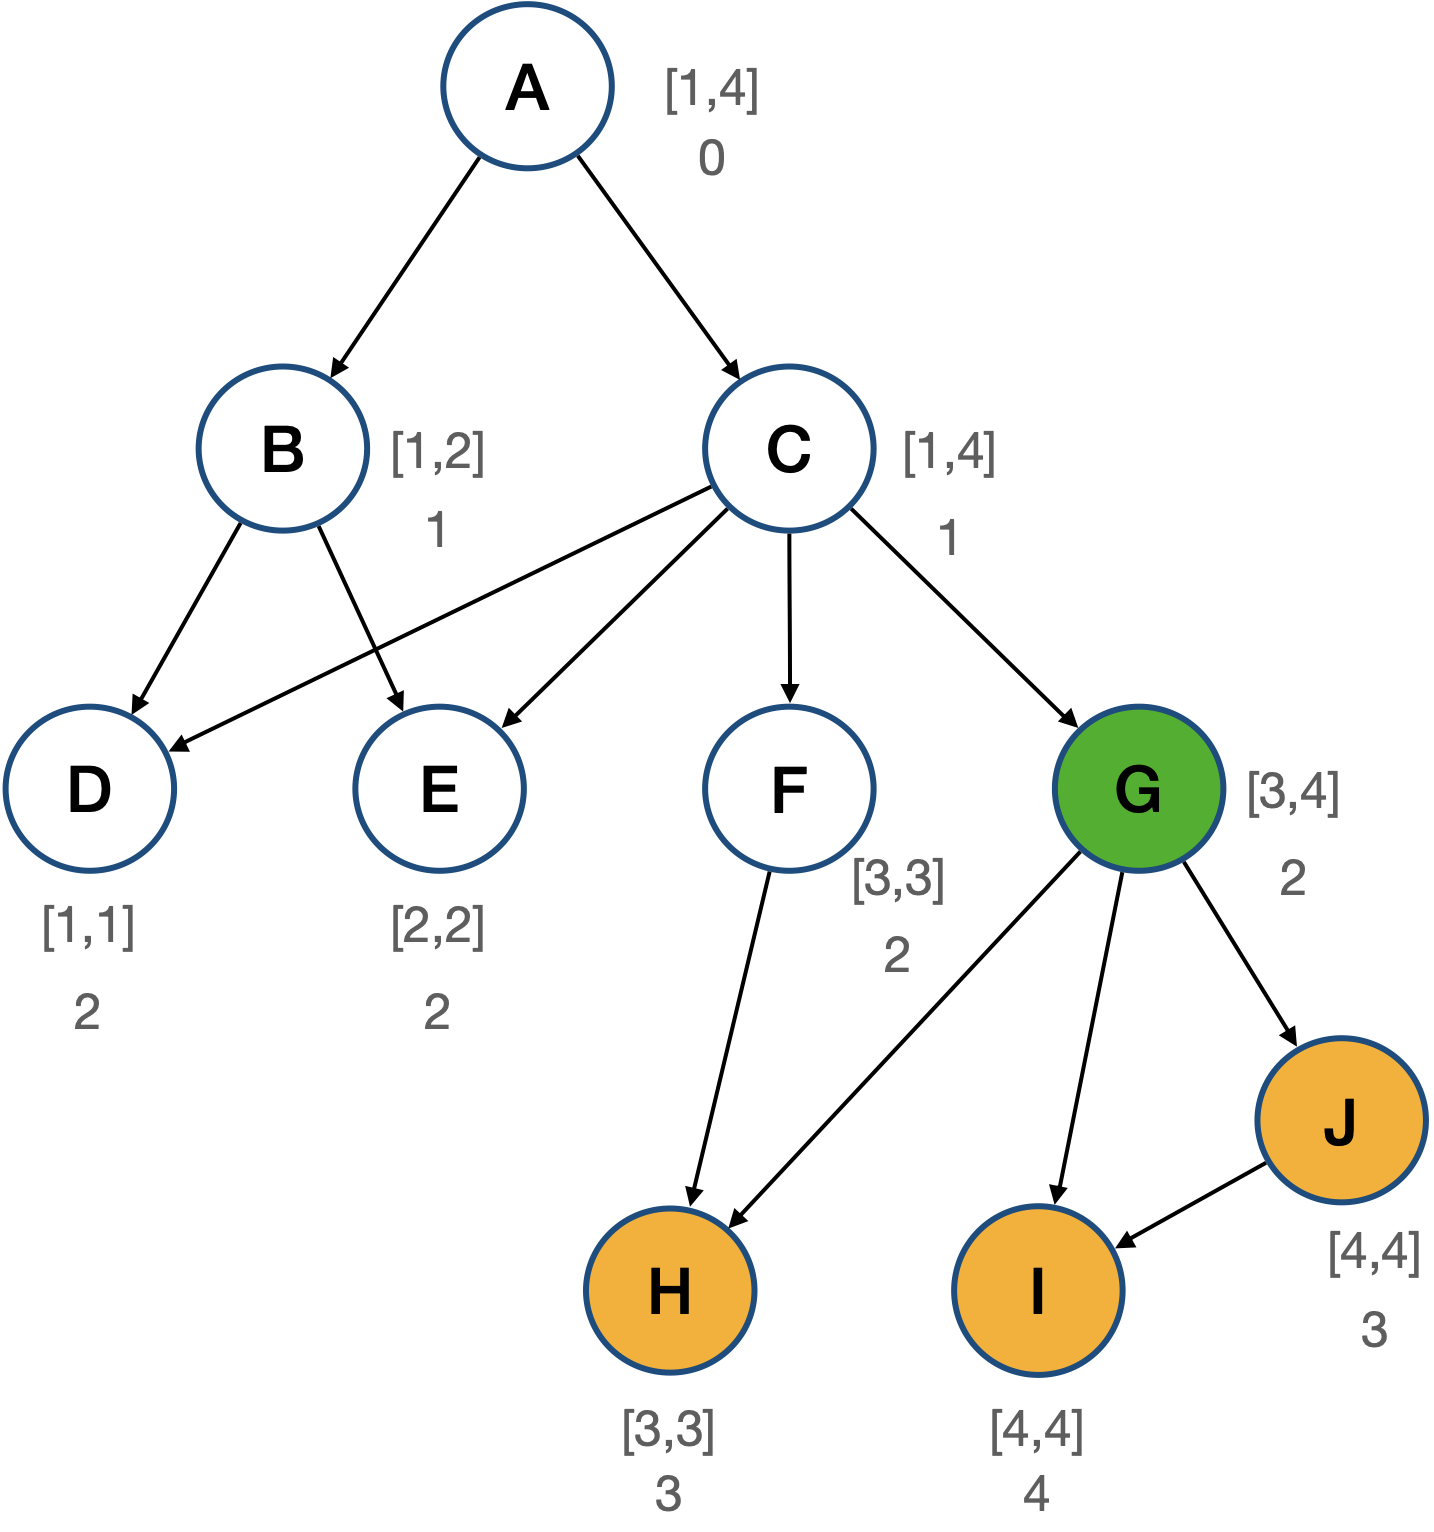
\includegraphics[width=0.5\textwidth]{figures/flexigran_example_with_lock.png}
    \caption{FlexiGran labels and vertex depth with lock on guard $G$ with the grain of the lock (yellow)}
    \label{fig:flexigran_example_locked}
\end{figure}

\subsection{Labelling through numeric intervals}
In FlexiGran, a post-order depth first traversal is performed to compute the labels of vertices. Like DomLock, the leaves of the hierarchy are labelled with unit intervals and internal vertices are labelled with intervals computed from the intervals of their children. In addition to these intervals, FlexiGran also computes the depth of each vertex in the hierarchy. The depth of a vertex is the length of the shortest-longest path from the root to the vertex. Figure \ref{fig:flexigran_example_locked} shows the intervals and vertex depths of a hierarchy labelled with FlexiGran.

This shortest-longest path is useful for depth determination in the presence of connected components like cycles. In a cycle, the path is recursive and based on the method of computation, the longest path can be infinite. The shortest-longest path breaks this recursion to a limit. This limit is the length of a path from the root to a vertex which contains the target vertex at most twice, as is the case with cycles. In a connected component, all the vertices have the same depth.  


\subsection{Lock Grain identification}
FlexiGran uses the depth information in addition to the intervals to determine the ancestor-descendant relationship between two vertices. Since both fine grained and MGL locks can exist in flexigran, the process of testing overlaps involves multiple tests. Table \ref{tab:flexigran_locks} shows the compatibility matrix for FlexiGran locks. When checking if two hierarchical locks are compatible, the intervals of their guards are tested for overlap. If the intervals are identical then the depth is used to break the tie and determine the ancestor-descendant relationship. 

\begin{table}[h]
    \centering
    \captionsetup{justification=centering}
    \begin{tabular}{c|cccc|cccc|}
        \multicolumn{1}{c}{} & \multicolumn{4}{c|}{\textbf{Lock On Ancestor}} & \multicolumn{4}{c}{\textbf{Lock On Descendent}} \\
        \cline{2-9}
        \textbf{Lock Mode} & \textbf{FR} & \textbf{FW} & \textbf{HR} & \textbf{HW} & \textbf{FR} & \textbf{FW} & \textbf{HR} & \textbf{HW} \\
        \hline
        \textbf{FR} & \cellcolor{green!25} Y & \cellcolor{green!25} Y & \cellcolor{green!25} Y & \cellcolor{red!25} N & \cellcolor{green!25} Y & \cellcolor{green!25} Y & \cellcolor{green!25} Y & \cellcolor{green!25} Y \\
        \textbf{FW} & \cellcolor{green!25} Y & \cellcolor{green!25} Y & \cellcolor{red!25} N & \cellcolor{red!25} N & \cellcolor{green!25} Y & \cellcolor{green!25} Y & \cellcolor{green!25} Y & \cellcolor{green!25} Y \\
        \textbf{HR} & \cellcolor{green!25} Y & \cellcolor{green!25} Y & \cellcolor{green!25} Y & \cellcolor{red!25} N & \cellcolor{green!25} Y & \cellcolor{red!25} N & \cellcolor{green!25} Y & \cellcolor{red!25} N \\
        \textbf{HW} & \cellcolor{green!25} Y & \cellcolor{green!25} Y & \cellcolor{red!25} N & \cellcolor{red!25} N & \cellcolor{red!25} N & \cellcolor{red!25} N & \cellcolor{red!25} N & \cellcolor{red!25} N \\
    \end{tabular}
    \caption{Flexigran compatibility matrix showing the protocol for the co-existence of hierarchical and fine-grained locks in a system. \textbf{F}: Fine-grained, \textbf{H}: Hierarchical, \textbf{R}:Read, \textbf{W}: Write}
    \label{tab:flexigran_locks}
\end{table}

When a hierarchical lock is tested for compatibility with a fine grained lock, then a traversal is performed to test the reachability of the fine grained lock guard from the hierarchical lock guard. If the fine grained lock guard is reachable from the hierarchical lock guard or vice-versa, then the two locks are incompatible. For example, in figure \ref{fig:flexigran_example_locked}, a hierarchical lock is acquired on $G$. This lock guards vertices $H$, $I$ and $J$. Unlike DomLock and MID, FlexiGran does not subsume $F$ since $F$ is not a descendant of $G$ since their depths are the same. In this situation, if a fine grained lock is requested on $F$, it would be compatible with the hierarchical lock on $G$ since there is no path from $G$ to $F$ or vice-versa.

\subsection{Label recomputation}
Like DomLock, structural modifications in FlexiGran require recomputation of the intervals of the vertices. A single depth first traversal is enough to recompute the intervals and depths of vertices. Since the root might be involved in the structural modification, a lock is placed on the root to prevent concurrent reads from interfering with the recomputation. This restricts concurrency and leads to a degradation in performance. 

As such, FlexiGran fulfils requirements $R1$ and $R2$ and incurs a significant performance penalty against requirement $R3$ due to the expensive compatibility checks required to detect conflicts between MGL and fine grained locks. FlexiGran also incurs a performance penalty against requirement $R4$ due to the non-parallel recomputation of intervals in dynamic hierarchies.


\section{Requirements and Trade-offs}
The different MGL techniques discussed in this chapter have tradeoffs. Recall the four primary requirements identified for MGL:
\begin{itemize}
    \item[\textbf{R1}] Identifying a lock guard for every vertex of a hierarchy.
    \item[\textbf{R2}] Finding an appropriate, optimal lock guard for a request.
    \item[\textbf{R3}] Detecting conflicts between locks i.e. testing ancestor-descendant relationship.
    \item[\textbf{R4}] Housekeeping the metadata required to implement the locking protocol.
\end{itemize}

\begin{figure}[h]
    \centering
    \captionsetup{justification=centering}
    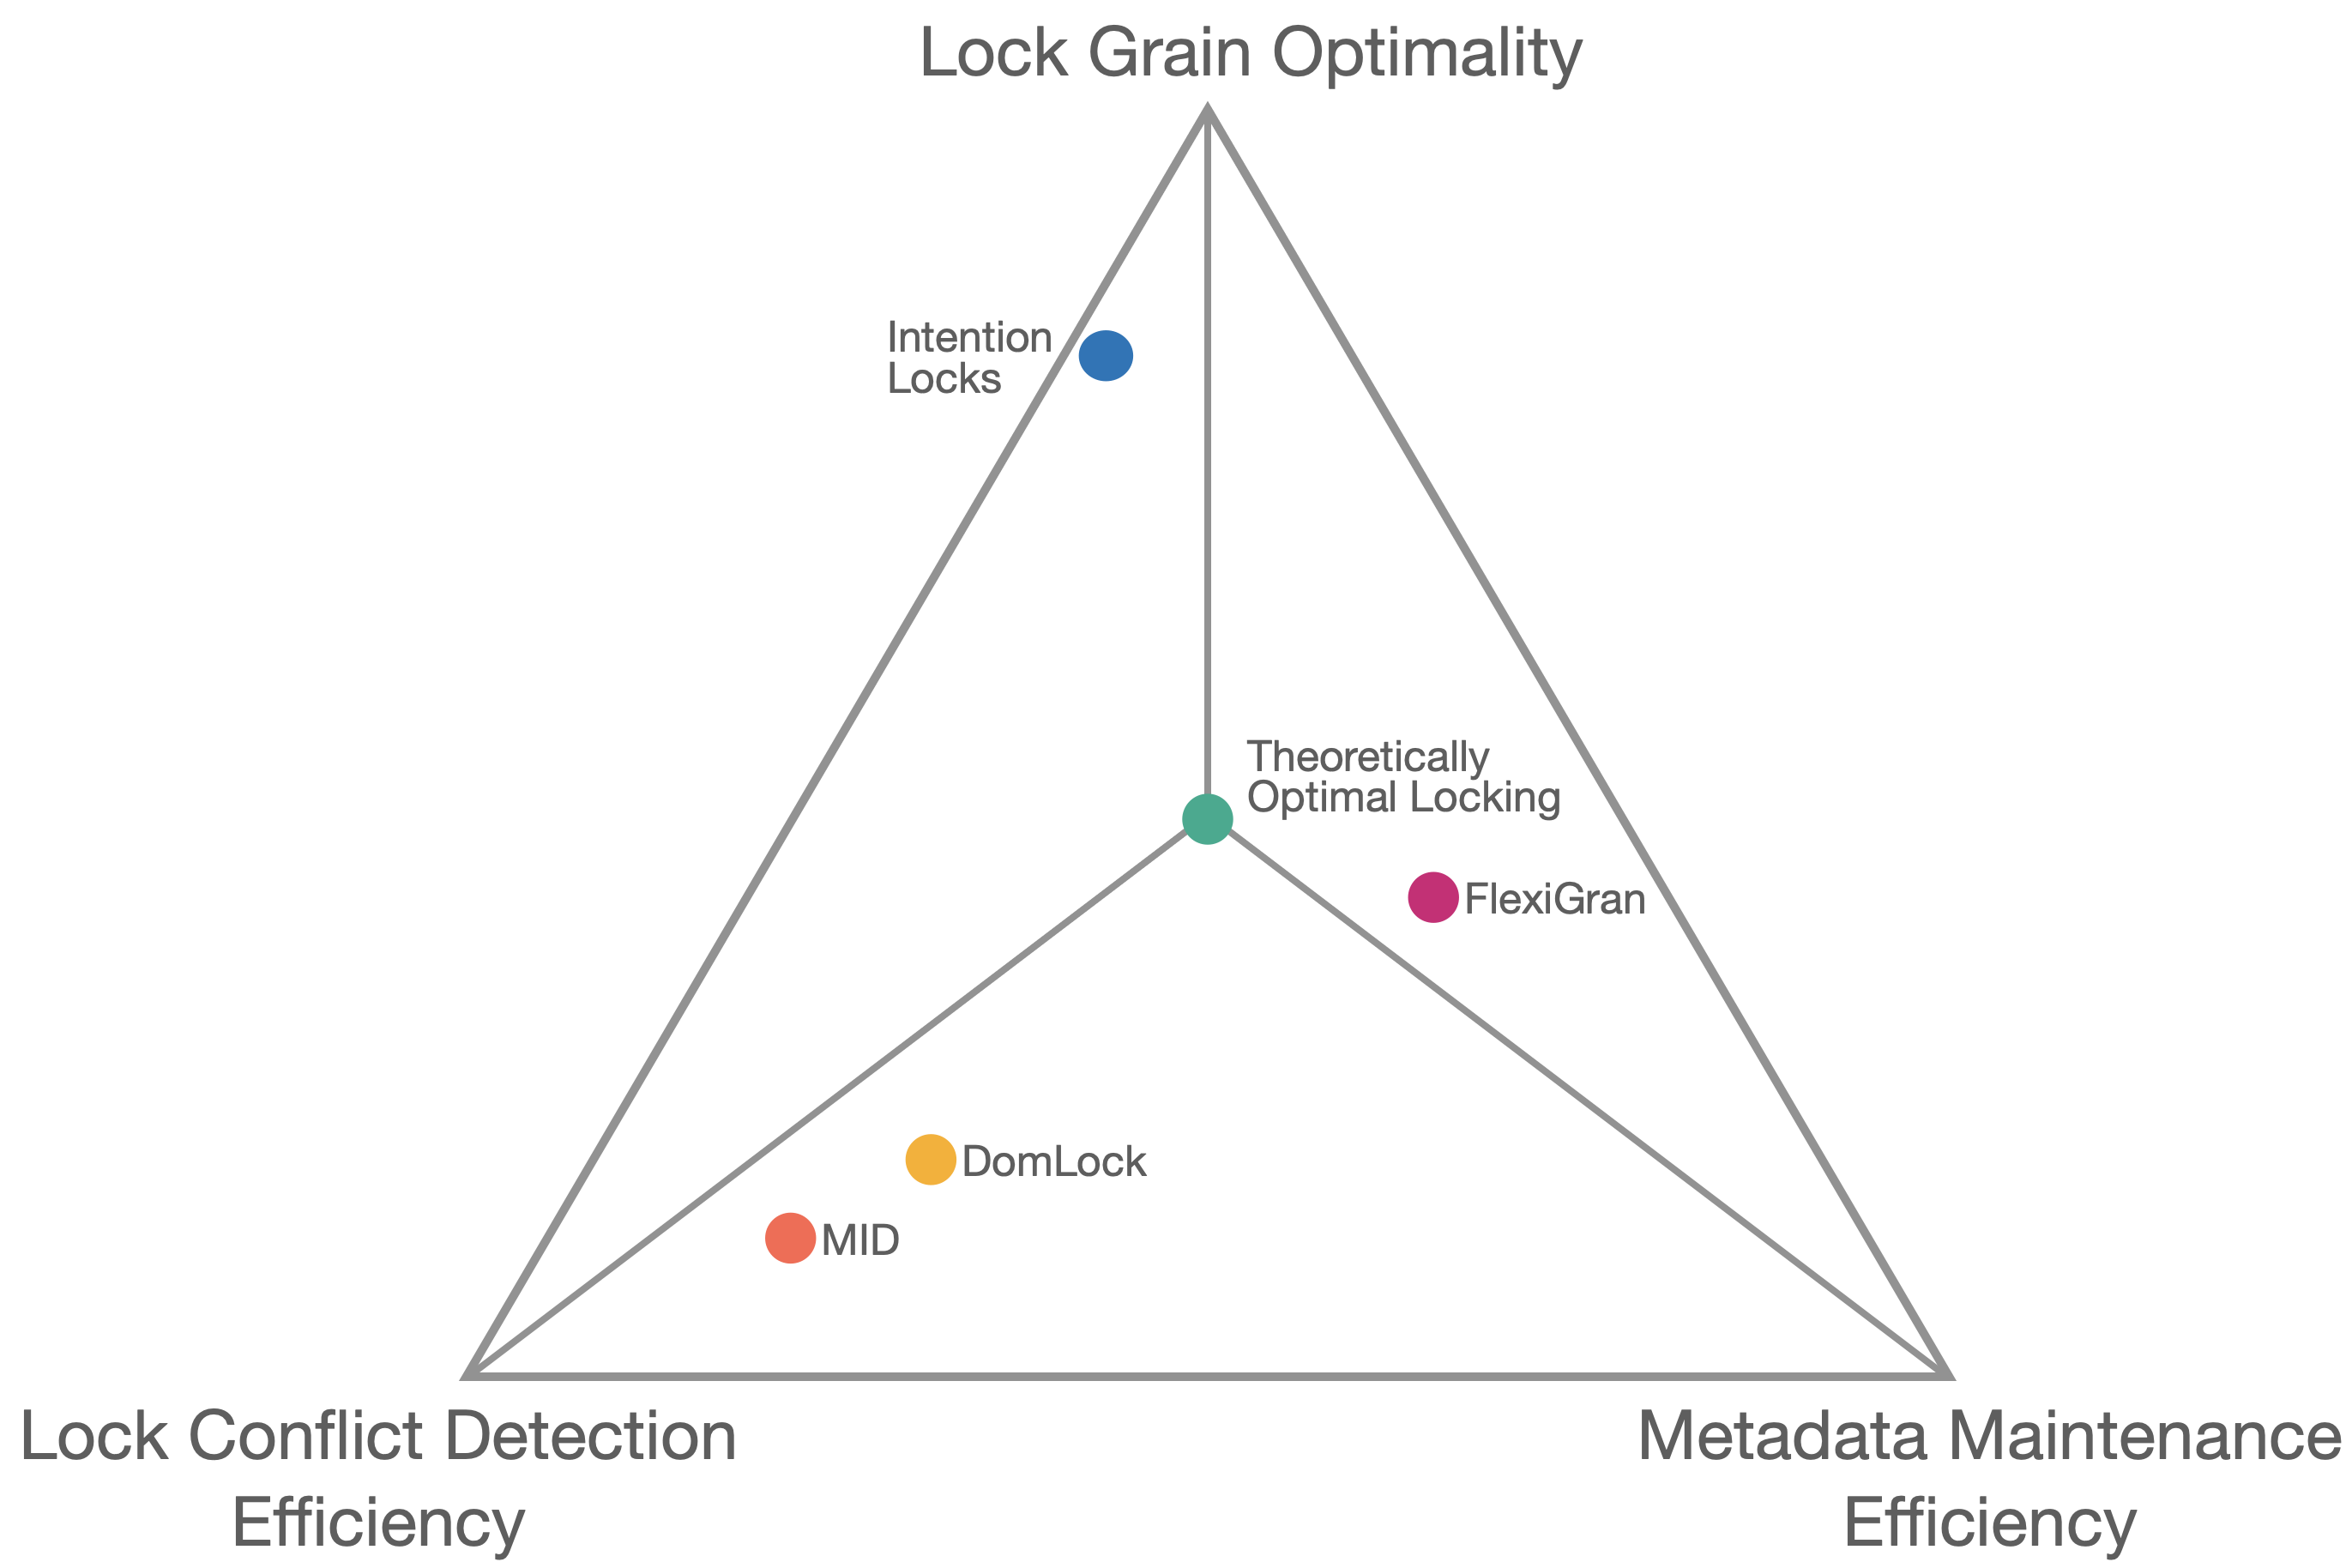
\includegraphics[width=.9\textwidth]{figures/MGL_comparision.png}
    \caption{Trade-offs in MGL techniques}
    \label{fig:tradeoffs}
\end{figure}

Fixed Grain locks are inefficient and only fulfil requirement \textbf{R1}. MGL based on traversals like Intention Lock, fulfils requirements \textbf{R1} and \textbf{R2} but incurs a significant performance penalty against requirement \textbf{R3} due to the sheer number of traversals required. 

Label based techniques like DomLock, MID also fulfil requirements \textbf{R1} and \textbf{R2} but incur a performance penalty against requirement \textbf{R3} due to false subsumptions. In addition, due to the metadata required to implement the locking protocol, these techniques incur a performance penalty against requirement \textbf{R4} as well. 

FlexiGran that implements MGL and fine grained locks suffer from poor performance due to the expensive compatibility checks and label recomputation. FlexiGran fulfils requirements \textbf{R1} and \textbf{R2} only. 

Figure \ref{fig:tradeoffs} shows the trade-offs in the different MGL techniques. Intention locks offer the most optimal lock grains at the cost of lock conflict detection efficiency. DomLock and MID offer efficient conflict detection at the cost of metadata management and do not have optimal lock grains. FlexiGran offers better lock grains but incurs a performance penalty due to the expensive lock conflict detection. None of the techniques balances all the requirements to come close to an optimal MGL protocol.

